\documentclass{beamer}
\usepackage{HECbeamer}
% \usepackage{pgfpages}
% \pgfpagesuselayout{4 on 1}[letterpaper, landscape, border shrink=5mm]
\title[\color{white}{MATH 60604A \S~7a -Censoring}]{\texorpdfstring{MATH 60604A \\Statistical modelling \\ \S~7a -Censoring}{MATH 60604A \\Statistical modelling \\ \S~7a -Censoring}}
\author{}
\institute{HEC Montréal\\
Department of Decision Sciences}
\date{} 

\begin{document}
\frame{\titlepage}
\begin{frame}
\frametitle{Survival data}
\begin{itemize} 
\item In \alert{survival analysis}, we're interested in the time until an event occurs, a non-negative response variable.
\item Let $T_i$ denote the \alert{survival time} for subject $i$ ($i=1, \ldots, n$).
\item The survival time is the amount of time that elapses before the event of interest occurs. 
\begin{itemize}
\vp \vp
\item Usually continuous, but often measured at discrete time values.
\item Survival time is also referred to as \alert{failure time} or \alert{time-to-event}.
\end{itemize}
\item Survival data itself is quite particular and it's critical to have a good understanding of the actual data in order to carry out an appropriate analysis.
\end{itemize}
\end{frame}

\begin{frame}
\frametitle{Examples of survival data }
Examples include
\begin{itemize}
\vp \vp
\item time until death for a patient diagnosed with cancer,
\item time until a patient is discharged from a hospital,
%\item time until a customer is seated at a restaurant
\item time until a customer cancels their gym membership,
\item time until an unemployed person finds a job,
\item time until a system fails.
\end{itemize}
\end{frame}

% 
% \begin{frame}
% \frametitle{Entry time}
% In order to define the survival time $T_i$, we must have a notion of the \alert{entry time} for the subject $i$. 
% \begin{itemize}
% \vp \vp
% \item That is, the time when $T_i=0$, when we start the stopwatch.
% \end{itemize}
% Entry time depends on the context of the study.
% \begin{itemize}
% \vp \vp
% \item It could be the same for all subjects: all subjects start at the same time.
% \begin{itemize} 
% \item time until a cohort of students starting in the Fall 2019 semester complete their degree
% \end{itemize}
% \item The entry time could vary from subject to subject, so they enter at different times. 
% \begin{itemize} \item time until a customer waiting in line is served.
% \end{itemize}
% \end{itemize}
% \end{frame}

\begin{frame}
\frametitle{Right-censoring}
% \begin{itemize}
% \item The variable of interest is the time $T$ until the event of interest happens.
% \item However, over the course of our study time frame, it might not be observed for all subjects. 
The biggest difficulty that arises when analyzing survival data is that \textbf{we don't necessarily observe all events}. 
\begin{itemize}
\vp \vp
\item the subject ``survives'' past the end of the study period
\bi
\item $T$ is the time until death after a patient is diagnosed with terminal cancer 
\bi 
\item could be that some patients are still alive at the end of the study period. \ei
\ei
\item the subject drops out of the study
\bi 
\item $T$ is the time it takes students to finish their degree 
\bi 
\item it could be that some students drop out of their program. \ei
\ei
\item a different event (or ``competing risk'') occurs which makes the event of interest impossible
\bi 
\item $T$ is the time until employees retire \bi \item it could be that an individual dies before being able to retire. 
\ei
\ei
\end{itemize}
% \end{itemize}
\end{frame}


\begin{frame}
\frametitle{Censoring}
 With censoring, the general idea is that we don't know the exact value of $T$, but we still have some information regarding some interval in which it could fall, e.g., $T>t$, or $T<t$, or $T \in [t_1,t_2]$

\begin{itemize}
\item \textbf{right censoring}: the event happens after some time $t$, i.e., $T_i \geq t$. 
\item \textbf{left censoring}: the event of interest has already occurred before the individual enters the study. That is, all we know is that $T<t$.
\item \textbf{interval censoring}: the event of interest occurs somewhere in an interval, but we don't know where exactly. That is, all we know is that $T \in [t_1,t_2]$
\end{itemize}
We will focus on the most common case, that of right censoring.


\end{frame}

\begin{frame}
\frametitle{Examples of censoring}
\begin{itemize} 
 \item Suppose a researcher is interested in studying the age at which children are able to write their names. 
\item Here, $T$ is the time (in years) until a child can write their name. 
\item The researcher follows children in a kindergarten class over the course of the school year. 
\begin{itemize}
\item 
When the researcher arrives, some children are already able to spell their name, in which case their time $T$ is \emph{left censored}. \item Some children learn to write their name while away during the Christmas Holidays, in which case their $T$ is \emph{interval censored}. 
\item Some children still don't know how to spell their name by the end of the school year, in which case their $T$ is \emph{right censored}.
\end{itemize}
\end{itemize}
\end{frame}


\begin{frame}
\frametitle{Non-informative censoring}
We typically assume that censoring is \alert{non-informative}. 
\begin{itemize}
\vp \vp
\item That is, the censoring time is independent of the survival time: it doesn't give us any information on what the survival time could be.
\end{itemize}
An example of \emph{informative} censoring:
\begin{itemize}
\vp \vp
\item Suppose a group of patients who are terminally ill are on an experimental treatment regime in which they are given some drug that could potentially have harmful side effects. However, for ethical reasons, patients who become very sick are taken out of the study. The patients who drop out will have $T$ that is right censored. However, those patients who drop out probably have poorer health to begin with and might be more likely to die sooner.
\end{itemize}

\end{frame}
\begin{frame}
 \frametitle{Non-informative right-censoring schemes}
 We distinguish between different types of right-censoring schemes:
 \begin{itemize}
  \item type 1 censoring: observations are collected until time $C$; all remaining observations are right-censored.
  \item type 2 censoring: we continue collection until $k$ events have been observed.
  \item \textbf{random censoring}: we observe $T_i = \min\{T_i^0, C_i\}$, where the time-to-event $T_i^0$ is independent of the censoring time $C_i$.
 \end{itemize}

\end{frame}
\begin{frame}
 \frametitle{Troncation}
 In certain studies, we collect data only during a time interval $[a, b]$. 
 \begin{itemize} 
 \item Survival time is \textbf{left-troncated} if survival time exceeds zero at time $a$
\end{itemize}
For example, during a unemployment survey, we could consider all people registered at the unemployment office between January and March. 
\begin{itemize} 
\item Some individuals lost their jobs before the year started and are already unemployed (left-truncation).
 \item If a person is still looking for a job at time $b$, the corresponding survival time will be right-censored (type I administrative censoring).
\end{itemize}
\end{frame}

\begin{frame}
\frametitle{Lexis diagram}
 \begin{center}
  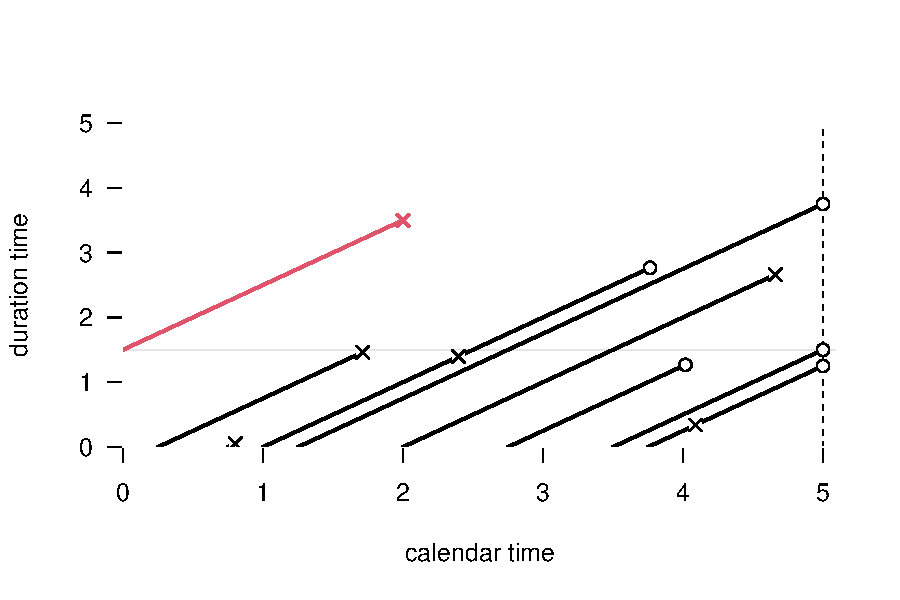
\includegraphics[width = 0.8\textwidth]{img/c7/07-lexis_en.pdf}
 \end{center}
{ \footnotesize A Lexis diagram represents the temporal trajectories of lifetime, with observed failure times denoted by $\mathrm{x}$ and right-censored observations by $\circ$. Residual observations at time $5$ are all censored. The trajectory in red corresponds to an individual whose survival time is left-truncated.

}
\end{frame}
\end{document}
